\section{Evaluation and results}\label{sec:11}

What follows is divided strictly into \textbf{what has been measured}, \textbf{what has been
proved}, and \textbf{what is pending}. The division is the point: an examiner should be able to
tell at a glance which claims are evidence and which are intent.

\subsection{Measured: the week-37 separation spike}\label{sec:11.1}

The kill criterion of the whole project was whether a residual separates a stuck damper from a busy
room at realistic sensor noise at all. The spike
(\texttt{project/spikes/residual-separation/}, plain Java 25, no dependencies, seeded and
reproducible bit for bit) simulated one 210 m³ room over 180 min, sampled at 60 s, with occupancy
stepping 0 → 10 people at $t = 10$ min and a damper command 20 \% → 80 \% at $t = 40$ min, at
$\sigma = 30$ ppm.

\begin{longtable}[]{@{}
  >{\raggedright\arraybackslash}p{(\columnwidth - 10\tabcolsep) * \real{0.14}}
  >{\raggedright\arraybackslash}p{(\columnwidth - 10\tabcolsep) * \real{0.14}}
  >{\raggedright\arraybackslash}p{(\columnwidth - 10\tabcolsep) * \real{0.12}}
  >{\raggedright\arraybackslash}p{(\columnwidth - 10\tabcolsep) * \real{0.20}}
  >{\raggedright\arraybackslash}p{(\columnwidth - 10\tabcolsep) * \real{0.14}}
  >{\raggedright\arraybackslash}p{(\columnwidth - 10\tabcolsep) * \real{0.26}}@{}}
\toprule
\textbf{Run (seed 42)} & \textbf{mean $r$} & \textbf{std $r$} & \textbf{mean $r$ after the
command} & \textbf{max CUSUM} & \textbf{crossing of $h$} \\
\midrule
\endhead
healthy & 3.5 ppm & 31.8 ppm & 5.3 ppm & 50.3 ppm & none \\
stuck & 392.1 ppm & 297.6 ppm & 507.8 ppm & 66\,996 ppm & $t = 47$ min, 7 min after the ignored
command \\
\bottomrule
\end{longtable}

The post-command mean residuals are \textbf{16.7 σ} apart. Over seeds 1–20: \textbf{20 of 20}
stuck runs crossed $h$, with delay min/median/max \textbf{5 / 8 / 11 min} against R-1's 15 min
budget, and \textbf{0 of 20} healthy runs crossed it. The healthy residual's standard deviation,
31.8 ppm, confirms that the injected noise is what reaches the residual and nothing else does.

The threshold sweep below is the R-1-against-R-3 trade-off, measured on those same 20 seeds (the
CUSUM statistic depends on $k$ only, so $h$ can be evaluated after the fact):

\begin{center}
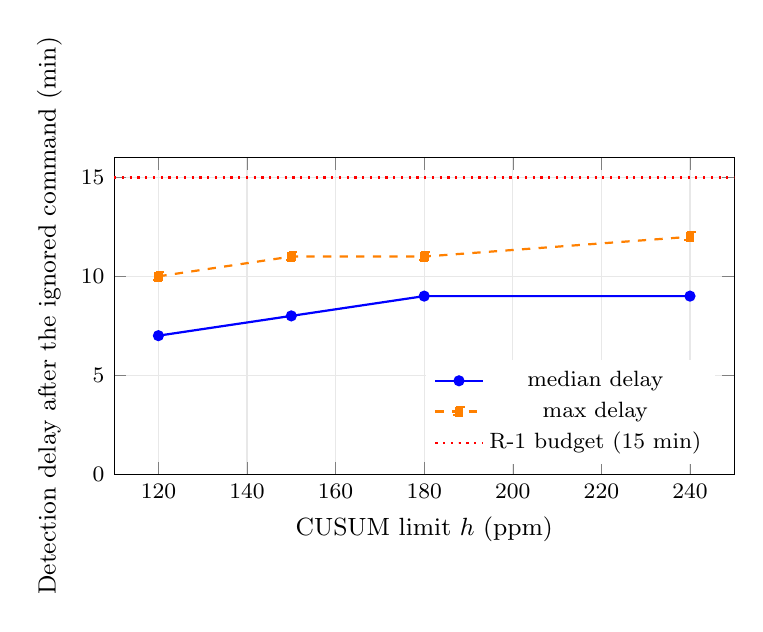
\begin{tikzpicture}
\begin{axis}[width=0.78\linewidth,height=5.6cm,
  xlabel={CUSUM limit $h$ (ppm)},ylabel={Detection delay after the ignored command (min)},
  xmin=110,xmax=250,ymin=0,ymax=16,legend pos=south east,
  legend style={font=\footnotesize,draw=none},grid=major,grid style={gray!18},
  tick label style={font=\footnotesize},label style={font=\small}]
\addplot[blue,thick,mark=*,mark size=1.6pt] coordinates {(120,7)(150,8)(180,9)(240,9)};
\addplot[orange,thick,dashed,mark=square*,mark size=1.6pt] coordinates {(120,10)(150,11)(180,11)(240,12)};
\addplot[red,dotted,thick] coordinates {(110,15)(250,15)};
\legend{median delay,max delay,R-1 budget (15 min)}
\end{axis}
\end{tikzpicture}
\end{center}
\figcap{Measured, from the spike's 20 seeds. Raising $h$ from 5σ (150 ppm) to 8σ (240 ppm) costs
about one minute of delay; lowering it to 4σ (120 ppm) already produced \textbf{1 false alarm in
20} three-hour healthy runs, while 5σ, 6σ and 8σ produced none. 150 ppm was chosen as the smallest
limit with no false alarm in the check set.}

\textbf{Two caveats bound every number above, and the spike's own result file states both.} The
observer used \emph{true occupancy}, so the healthy residual was pure sensor noise with no model
error, which makes 0 of 20 an optimistic bound. And the worst healthy seed peaked at
\textbf{149.1 ppm against $h$ = 150 ppm} (a 0.9 ppm margin, with the next-highest seed at
91.6 ppm), so the clean check set is a tail draw rather than a design property. R-3 asks the same
statistic to hold over seven days and six rooms, which is far more samples, and \textbf{the margin
did not survive that horizon}: §\ref{sec:11.2} measures \textbf{0.55} confirmed cases per fault-free week with
a \textbf{worst week of 6} against R-3's limit of one. The tuning is therefore no longer merely
reported: it is measured, and it fails. \textbf{Appendix \ref{sec:F.1}} gives both caveats in full, with
ADR-0010's attribution of why the margin was so thin; it was not the limit, which is why $k$ and $h$
are left where the spike put them rather than retuned (§\ref{sec:13.4}).
\subsection{Measured: the evaluation harness, R-1 to R-7}\label{sec:11.2}

The harness in \texttt{project/evaluation/} drives the same control and diagnosis classes the
containers run (\texttt{BuildingSimulation}, \texttt{DcvControlLoop}, \texttt{FaultMonitor},
\texttt{SupervisionService}) in one JVM against a simulated clock, with events handed between them
directly instead of through the broker and the journal replaced by a counter. One full run on
OpenJDK 25.0.3, Mac OS X on aarch64, takes 350 s of wall clock over \factExperiments{} experiments and writes nine
result tables. Every number in this subsection is read off that run, which was taken after all of
this session's changes had merged. So no figure here comes from a run of a subset of the code.

\begin{longtable}[]{@{}
  >{\raggedright\arraybackslash}p{(\columnwidth - 6\tabcolsep) * \real{0.07}}
  >{\raggedright\arraybackslash}p{(\columnwidth - 6\tabcolsep) * \real{0.09}}
  >{\raggedright\arraybackslash}p{(\columnwidth - 6\tabcolsep) * \real{0.56}}
  >{\raggedright\arraybackslash}p{(\columnwidth - 6\tabcolsep) * \real{0.28}}@{}}
\toprule
\textbf{Req.} & \textbf{Run} & \textbf{Measured} & \textbf{Verdict} \\
\midrule
\endhead
R-1 & T-24 & Stepped protocol, 20 seeds, $h$ = 150 ppm: 20/20 detected at 4 / 6 / 6 / 7 min
(min / median / p95 / max) against a 15 min budget, and p95 between 5 and 8 min over
$h$ = 50…300 ppm. Closed loop on a drawn weekday at the same $h$: 15/20 detected, 21 / 74 / 257 /
257 min & \textbf{Met as specified; not met in closed loop} \\
R-2 & T-26 & Fraction of occupied minutes at or below 1000 ppm after onset, 5 seeds. Drawn weekday
1.000, 5 of 5 seeds, unchanged with the lower CUSUM arm off and with no damper feedback. Every room
at design occupancy: 0.022 supervised against 0.009 unsupervised (\textbf{0 of 5 seeds}),
while the no-fault reference is 1.000 and 5 of 5 in every case & \textbf{Met on the case it
covers; not met at design occupancy} \\
R-3 & T-25 & Distinct confirmed cases per fault-free week over 20 simulated weeks of all six rooms:
\textbf{0.55 per week} against a limit of 1, \textbf{16 of 20 weeks clean}, worst week 6 (1.30 per
week with 9 clean weeks before ADR-0010). The scored criterion is the worst week & \textbf{Not met} \\
R-4 & T-27 & Each component killed in turn in one JVM, \textbf{23 of 23 assertions}: every
observable room \texttt{BLIND} within 4 cycles, 0 fault events while blind, 0 damper commands on
stale data, \texttt{HEALTHY} 3 cycles after readings return. \textbf{The container-level run has
since been done}: five of six rooms \texttt{BLIND} within 12 s against \texttt{docker compose},
three-cycle recovery, restart policy firing on an in-container \texttt{SIGTERM} & \textbf{Met
in-JVM and at container level} \\
R-6 & T-28 & 25\,600 zones at a p95 of about 6 s (5.68–6.05 s over five runs), inside the 60 s
interval; fitted over the nine points from 100 zones up,
p95 = $1.196\times10^{-8}\,n^{1.97}$ s with $r^2$ = 0.9991; the crossing of 60 s extrapolated at
$\approx$ 86\,000 zones; saturated element \texttt{AhuFlowModel.believedFlowTo}, $\Theta(n^2)$ per
cycle. \textbf{The deployed ceiling is a different and far smaller number}: 58 zones, bounded by
BuildSim's floorplan rather than by the monitor & \textbf{Met in the harness}, and the two ceilings
are never quoted as one \\
R-7 & T-34b & Injected room rotated over all six rooms, 3 seeds, 3 configurations, in \emph{two
occupancy regimes}, 540 observed rooms. Drawn weekday, 270 rooms: \textbf{0 failed}, airflow inside
the 5 \% tolerance everywhere. Design occupancy, 270 rooms: \textbf{231 failed} (215 accused of a
fault they did not have, 16 more outside the airflow band at a worst 0.058919, the two sets
disjoint); 40 rooms reached \texttt{COMPENSATING} and \textbf{130 of the 215 falsely latched rooms
reached \texttt{DEGRADED}}. The supervisor does not merely accuse those rooms, it takes their
dampers off the inner loop & \textbf{Met on the drawn weekday; not met at design occupancy} \\
\bottomrule
\end{longtable}
Six of the seven requirements are scored in that table; \textbf{R-5's evidence is a live rebuild
rather than a harness experiment}, reported with the journal in §\ref{sec:5} and in Appendix \ref{sec:G}.

\textbf{Two readings of the table matter more than any single row.} The first is that \textbf{every
failing verdict above is a regime statement, not a global one}: R-1 is met on the stepped protocol
its own verification column names and fails in closed loop; R-2 is met on the drawn weekday and
fails with every room at design occupancy; R-7 is met on 270 drawn-weekday observed rooms and fails
on 231 of 270 at design occupancy. Quoting either arm without the other misrepresents the result, so
this report never does. The second is that \textbf{R-3 is not one failing requirement among four; it
is the one whose failure the other three inherit.} R-2's design-occupancy seeds fail partly because
false alarms have already latched rooms that would otherwise have been healthy dampers to trim
(R-3's false alarms consume the lever R-2 depends on), and the larger half of R-7's failure is 215
observed rooms accused of a fault they did not have, which is R-3's rate arriving inside another
requirement's experiment in a regime R-3's own replay never visits.

\textbf{Appendix \ref{sec:F.3} carries the working behind every verdict}: what separates protocol from
occupancy in R-1's two arms, the stratification of T-24's 20 drawn weekdays, T-25's baseline contest
and T-29's learned contender with the operating point attached to each ratio, R-2's five seeds and
the lever each plan ran out of, R-3's 26 pre-fix confirmations classified by arm and cause with the
half of the fix that was declined on evidence, R-6's fit and its two ceilings, and R-7's two
disjoint failing clauses with the supervisor-dead pass that separates them.

\subsection{Proved: compensation holds the healthy rooms exactly}\label{sec:11.3}

This result is analytic and pinned by unit tests, not produced by an experiment, and it is
presented as such. The per-room flows below follow from Section \ref{sec:7.4}'s closed form at Section \ref{sec:6}'s
parameters: five healthy dampers at 0.60, A145's frozen at 0.15, baseline fan 0.70, trim
$t = 0.360$, fan raised to $s = 0.880$.

\begin{center}
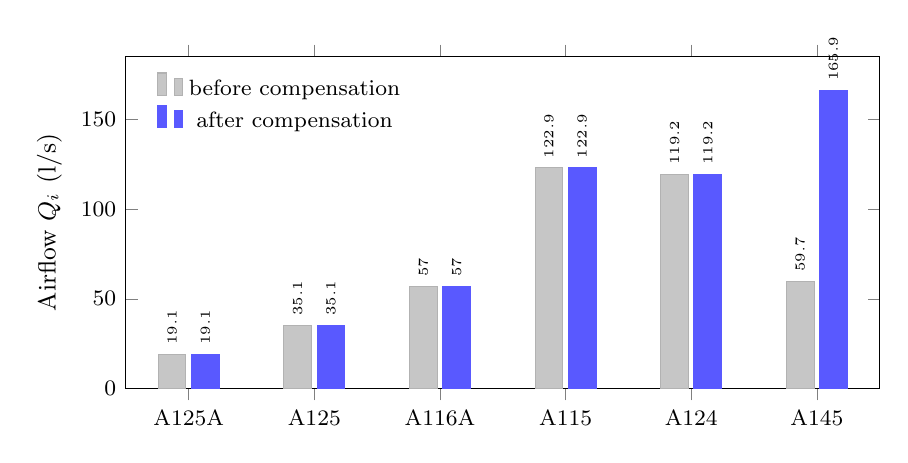
\begin{tikzpicture}
\begin{axis}[width=0.92\linewidth,height=5.8cm,ybar,bar width=10pt,
  ylabel={Airflow $Q_i$ (l/s)},ymin=0,ymax=185,
  symbolic x coords={A125A,A125,A116A,A115,A124,A145},xtick=data,
  legend pos=north west,legend style={font=\footnotesize,draw=none},
  nodes near coords,every node near coord/.append style={font=\tiny,rotate=90,anchor=west},
  enlarge x limits=0.10,tick label style={font=\footnotesize},label style={font=\small}]
\addplot[fill=gray!45,draw=gray!60] coordinates {(A125A,19.1)(A125,35.1)(A116A,57.0)(A115,122.9)(A124,119.2)(A145,59.7)};
\addplot[fill=blue!65,draw=blue!65] coordinates {(A125A,19.1)(A125,35.1)(A116A,57.0)(A115,122.9)(A124,119.2)(A145,165.9)};
\legend{before compensation,after compensation}
\end{axis}
\end{tikzpicture}
\end{center}
\figcap{Computed from the solver's closed form, and asserted by
\texttt{CompensationSolverTest}. A145, frozen at its 0.15 damper floor, goes from 59.7 l/s to
165.9 l/s (its full design flow, a gain of 2.78), while the five healthy rooms' flows are
unchanged to within $10^{-15}$. This is arithmetic that closes exactly, not a measurement; the
closed-loop CO₂ that is R-2's actual criterion is measured separately, and §\ref{sec:11.2} reports where it
holds and where it does not.}

\begin{longtable}[]{@{}
  >{\raggedright\arraybackslash}p{(\columnwidth - 6\tabcolsep) * \real{0.2870}}
  >{\raggedright\arraybackslash}p{(\columnwidth - 6\tabcolsep) * \real{0.1722}}
  >{\raggedright\arraybackslash}p{(\columnwidth - 6\tabcolsep) * \real{0.1722}}
  >{\raggedright\arraybackslash}p{(\columnwidth - 6\tabcolsep) * \real{0.3636}}@{}}
\toprule
\textbf{Case} & \textbf{Trim $t$} & \textbf{Gain achieved} & \textbf{Healthy flow deviation} \\
\midrule
\endhead
Requested gain 2.0, fan at 0.70 & 0.500 & exactly 2.000 & \textbf{0}, fan raised to 0.8012 \\
Restore A145 to design flow, fan at 0.70 & 0.360 & 2.779 & \textbf{0}, fan raised to 0.880 \\
Requested gain 4.0, fan \emph{already} at 1.00 & 0.733 & \textbf{1.296 only} & exactly 5 \%, the
stated tolerance; the fan has nothing left to raise \\
Damper stuck fully shut & no trim & \textbf{none} & no command issued; critical work order instead
\\
\bottomrule
\end{longtable}

The third row is the honest one and the most useful: with the fan already saturated (peak
occupancy, or a blocked filter the inner loop has already answered with speed), compensation
delivers a gain of \textbf{1.296, not 4}, and buys even that by taking exactly 5 \% from each
healthy room. Flow is redistributed, not created. Reporting R-2 without that bound, and without the
stuck-shut bound, would misrepresent it: the claim this design supports is not ``the system keeps
faulted rooms breathable'' but ``it does so while the damper still passes 15 \% of its design
opening and the fan has headroom''.

\subsection{Proved: architectural properties}\label{sec:11.4}

These are properties of code rather than of physics, and a simulator is the right instrument for
them. Each is covered by unit tests in the control and entity layers: that
\texttt{fault-monitor} never writes an actuator topic; that an aggregate cannot be constructed in
an illegal state (a \texttt{FanSpeed} outside $[0.2, 1.0]$, a damper position outside $[0,1]$);
that a latched \texttt{FaultCase} leaves \texttt{CONFIRMED}/\texttt{COMPENSATING} only through
\texttt{serviced()}; that \texttt{BLIND} has no edge into an open case; and that a zone in
\texttt{DEGRADED} mode receives no normal control command.

\subsection{Not measured: what the numbers above do not say}\label{sec:11.5}

The detector is evaluated against its own generator. \texttt{physics-simulator} freezes a damper,
scales flow by $(1-\beta)$ or adds a sensor offset, and \texttt{fault-monitor} looks for exactly
those three things using the same mass balance and the same flow split. \textbf{Every detection
result is therefore a measurement of self-consistency between two pieces of one person's
arithmetic.} The p95 delay (R-1), the false-alarm rate (R-3) and the comfort percentile (R-2) are
conditional on the generator: they describe how this detector behaves against this fault
definition, and say nothing about a real air handler. Section \ref{sec:13.2} develops this.

A second, sharper limit on what can be claimed, and T-15 has since made it sharper still: of the
faults the project set out to name, \textbf{one is classified and the others can only be pointed at}.
\texttt{STUCK\_DAMPER} is the reliable one, and T-24, T-25, T-26 and T-34b are all measurements of
it. \texttt{BLOCKED\_FILTER}'s branch is \textbf{unreachable with this physics} for structural
reasons §\ref{sec:13.1} sets out: it confirms as \texttt{UNCLASSIFIED} with its plant power excess reported,
which is the right behaviour for a case the system cannot prove. And \texttt{SENSOR\_DRIFT} is
\textbf{never emitted at all} (0 of 76 runs from a drift ramp and 0 of 76 from a step offset),
so the room is named a stuck damper instead: a confident, specific, wrong work order rather than an
honest \texttt{UNCLASSIFIED}. \textbf{Appendix \ref{sec:D.3}} records why that is a property of the classifier
rather than of the generator, an attribution this report had the wrong way round until the experiment
was run.

\subsection{Every pending measurement, in one place}\label{sec:11.6}

\textbf{Every row of that register is now filled, and no row is filled with an estimate.} What was a
fourteen-row table of pending measurements is seven rows of experiments that have all run: T-24's
occupancy stratification, T-20's live case rebuild, T-27's container kills, T-15's confusion matrix
over 218 runs, T-29's optional learned contender (\textbf{measured and dropped}), T-23's
dashboard frames, and T-35's reordering of the diagnosis (\textbf{measured and not adopted}). Each
row keeps the bound on what its evidence actually is.

\textbf{The table being full is not the same as every requirement passing}: R-1 and R-3 still fail on
the arms §\ref{sec:11.2} names, R-2 and R-7 fail on the harder of their two occupancy regimes, and one of four
injected mechanisms is classified. \textbf{Appendix \ref{sec:G}} is the register row by row, with one result the
obvious experiment measures wrongly: a \texttt{docker kill} cannot tell a working restart policy
from a missing one, because the daemon records it as a manual stop.

\subsection{Measured: what the compensation costs in energy}\label{sec:11.7}

This is the last measurement folded in, which is why it sits after the register rather than among
its siblings. It needed no new experiment: both halves are columns of
\texttt{evaluation/results/T-26-comfort.csv}, the same five-seed run §\ref{sec:11.2} scores R-2 from, read
together for the first time.

Fan power follows the affinity law, $P \propto s^3$ (§\ref{sec:6}, Appendix \ref{sec:E}), so the second lever is priced
superlinearly while the airflow it buys is not. The question that makes it a sustainability result
rather than an arithmetic one is what the system actually spent, per regime, against what the
spending bought.

\begin{longtable}[]{@{}
  >{\raggedright\arraybackslash}p{(\columnwidth - 8\tabcolsep) * \real{0.26}}
  >{\raggedright\arraybackslash}p{(\columnwidth - 8\tabcolsep) * \real{0.17}}
  >{\raggedright\arraybackslash}p{(\columnwidth - 8\tabcolsep) * \real{0.19}}
  >{\raggedright\arraybackslash}p{(\columnwidth - 8\tabcolsep) * \real{0.19}}
  >{\raggedright\arraybackslash}p{(\columnwidth - 8\tabcolsep) * \real{0.19}}@{}}
\toprule
\textbf{Regime} & \textbf{Comfort, no supervisor} & \textbf{Comfort, supervisor} & \textbf{Mean
plan fan speed} & \textbf{Fan power vs normal} \\
\midrule
\endhead
Drawn weekday & 1.0000 & 1.0000 & \textbf{0.7000} & \textbf{×1.00} \\
Design occupancy & 0.0094 & 0.0217 & 0.8171 (max 1.0000) & \textbf{×1.59} (max ×2.92) \\
\bottomrule
\end{longtable}

\textbf{The result is the shape of those two rows, not either number on its own.} On the drawn
weekday, the regime where R-2 is met, the plan's fan speed is \textbf{0.7000 in all five
seeds}: the common trim on the healthy dampers covers the whole requested gain and \emph{the raise
is never spent at all}. Compensation there is free. At design occupancy it costs on average
\textbf{1.59 times the fan power}, and up to 2.92 times where no healthy room is left to
over-supply, to move occupied comfort minutes from 0.0094 to 0.0217: a gain of
\textbf{0.0123 against an acceptance criterion of 0.95}.

So the energy is spent almost exactly where it does least good, and that is a property of the
\emph{plant}, not of the control law. The ceiling is the damper floor and the fan curve: when every
room is generating CO\textsubscript{2} at design rate, there is no healthy room with spare airflow
to trim, the solver falls back on the one lever that remains, and that lever is the cubed one.
\textbf{Buying 1.2 \% of comfort minutes for 59 \% more fan energy is not a trade worth making},
and the honest conclusion is that at design occupancy the supervisor should \emph{decline} to
compensate and say so in the work order, which is what the stuck-shut case already does, where
the plan reports ``no air path'' and the narrative turns to occupancy advice (§\ref{sec:7.4}, Appendix \ref{sec:E})
rather than spending the fan on a room it cannot reach.

That change is not made here. It would alter R-2's measured arm two days before this document was
frozen, and a requirement that fails for a mechanism this report can name is better evidence than
one that passes because the experiment was changed after the result was known. It is recorded in
§\ref{sec:13} as the first thing to do next, with the number that justifies it.
